\documentclass[UTF8,fontset=none,12pt]{ctexart}

\setCJKmainfont{Songti SC}
\setCJKsansfont{PingFang SC}
\setCJKmonofont{Songti SC}

\usepackage[a4paper,margin=2.35cm]{geometry}
\usepackage{amsmath,amssymb,amsthm,mathtools,bm}
\usepackage{graphicx}
\usepackage{float}
\usepackage{booktabs}
\usepackage{array}
\usepackage{enumitem}
\usepackage[hidelinks]{hyperref}

\title{数值线性代数\quad 第 30 讲：其他特征值算法}
\author{Lloyd N. Trefethen、David Bau III\quad 中文阅读版}
\date{}

\begin{document}
\maketitle
\pagestyle{plain}

特征值的计算并不只有 QR 算法。本讲简要介绍实对称特征值问题的三个著名替代
方法：适用于满矩阵的 Jacobi 算法，以及适用于三对角矩阵的二分法和分治算法。

\section*{Jacobi 算法}

计算矩阵特征值的最古老思想之一是 Jacobi 算法，它由 Jacobi 于 1845 年提出。
整个计算机时代，这个方法一直受到关注，尤其是在并行计算出现以后；不过它始终
没有完全取代其他方法。

想法如下。对于维数至少为 5 的矩阵，我们知道特征值只能通过迭代得到（第 25 讲）。
但更小的矩阵可以一步处理。既然如此，为什么不先对 $A$ 的一个小子矩阵对角化，
再对另一个小子矩阵对角化，如此反复，希望最终得到整个矩阵的对角化呢？

有人尝试过使用 $4\times4$ 子矩阵，但标准方法基于 $2\times2$ 子矩阵。一个
$2\times2$ 实对称矩阵可以写成

\begin{equation}
J^T\begin{bmatrix}a&d\\d&b\end{bmatrix}J
 =\begin{bmatrix} *&0\\0&*\end{bmatrix},
\qquad J\text{ 为正交矩阵}.
\tag{30.1}
\end{equation}

选择 $J$ 有几种方式。一种方式是取 $2\times2$ Householder 反射

\begin{equation}
F=\begin{bmatrix}-c&s\\s&c\end{bmatrix},
\qquad s=\sin\theta,\quad c=\cos\theta.
\tag{30.2}
\end{equation}

注意 $\det F=-1$，这正是反射的标志。另一种方式是不使用反射，而使用旋转

\begin{equation}
J=\begin{bmatrix}c&s\\-s&c\end{bmatrix},
\qquad \det J=1.
\tag{30.3}
\end{equation}

Jacobi 算法采用后一种标准做法。可以证明，只要 $\theta$ 满足

\begin{equation}
\tan(2\theta)=\frac{2d}{b-a},
\tag{30.4}
\end{equation}

就能实现 (30.1) 的对角化。按此选择构造的矩阵 $J$ 称为 Jacobi 旋转。它与
Givens 旋转（习题 10.4）的形式相同；唯一差别是，$\theta$ 的选择目标是使
$J^TAJ$ 对角，而不是使 $J^TA$ 三角化。

现在令 $A\in\mathbb{R}^{m\times m}$ 为对称矩阵。Jacobi 算法就是反复应用基于
(30.3)、(30.4) 构造的变换 (30.1)。此时把 $J$ 扩展为 $m\times m$ 矩阵，除
四个条目外其余部分都是单位矩阵，而那四个条目构成 (30.3)。左乘 $J^T$ 会
修改 $A$ 的两行，右乘 $J$ 会修改 $A$ 的两列。每一步都会在矩阵中引入一对
对称位置的零，但之前的零也会被破坏。不过，和 QR 算法一样，这些非零条目的
绝对值通常会持续缩小。

每一步应该把哪个非对角条目 $a_{ij}$ 消成零？最适合手算的做法是每次选择
绝对值最大的非对角条目。这样收敛分析几乎是直接的：可以证明，每一步非对角
条目平方和至少缩小为原来的

$$
1-\frac{2}{m^2-m}
$$

（见习题 30.3）。经过 $O(m^2)$ 步、每步需要 $O(m)$ 次运算后，平方和必然
缩小一个常数因子；因此要达到 $\varepsilon_{\mathrm{machine}}$ 的精度，需要

$$
O\!\left(m^3\log\frac{1}{\varepsilon_{\mathrm{machine}}}\right)
$$

次运算。事实上，已知其收敛性比这个估计更好，最终是二次收敛而不是线性收敛，
所以实际运算量为

$$
O\!\left(m^3\log\left|\log\varepsilon_{\mathrm{machine}}\right|\right)
$$

（见习题 25.2）。

在计算机上，通常按循环顺序消去非对角条目，从而避免 $O(m^2)$ 的“寻找最大值”
操作。例如，若按行顺序从 $a_{12},a_{13},\ldots$ 开始消去
$m(m-1)/2$ 个上三角非对角条目，就仍能保证快速的渐近收敛。对全部
$m(m-1)/2$ 对非对角条目完成一轮 $2\times2$ 操作后，精度通常已经提高了
一个超过常数因子的幅度；而且收敛最终仍为二次。

Jacobi 方法很有吸引力，因为每次只处理一对行和一对列，因而很容易并行化
（见习题 30.4）。它不需要预先把矩阵约化为三对角形式；事实上，Jacobi 旋转
会破坏三对角结构。对于 $m\le1000$ 的矩阵，通常不到十轮扫描就能收敛，最终
的逐元素精度一般甚至优于 QR 算法。不过，即使在并行计算机上，Jacobi 算法
通常也不如“三对角化再接 QR 或分治算法”（下文讨论）快，但通常只慢一个数量级
以内（见习题 30.2）。

\section*{二分法}

下一个特征值算法二分法具有很大的实际意义。对对称矩阵完成三对角化后，如果
不需要全部特征值而只需要其中一部分，二分法就是标准的后续步骤。例如，它可以
找出最大的 $10\%$ 特征值、最小的 30 个特征值，或者区间 $[1,2]$ 中的全部
特征值。找到所需特征值后，可以用一次逆迭代（算法 27.2）得到相应的特征向量。

出发点很初等。由于实对称矩阵的特征值都是实数，我们可以在实轴上寻找多项式

$$
p(x)=\det(A-xI)
$$

的根。这听起来像一个坏主意：第 15 讲和第 25 讲不是说过，从多项式系数出发
求根是计算特征值的高度不稳定过程吗？区别在于，前面的批评针对的是“从多项式
系数求根”。现在的想法是在不同的点 $x$ 直接计算 $p(x)$，完全不接触它的系数，
然后对这个非线性函数应用通常的二分过程。例如，可以通过带主元的高斯消去法
（习题 21.1）完成函数值计算；所得算法会具有很高的稳定性。

这听起来已经很有用，但还不算特别令人兴奋。二分法真正强大且吸引人的地方，
是特征值和行列式还具有一些不那么直接的额外性质。

令对称矩阵 $A\in\mathbb{R}^{m\times m}$ 的 $A^{(1)},\ldots,A^{(m)}$ 表示其
维数分别为 $1,\ldots,m$ 的主子矩阵（即左上角方形子矩阵）。可以证明这些矩阵
的特征值彼此交错。在定义这一性质前，先作一个更强的假设：$A$ 是三对角矩阵，
并且不可约，即所有非对角线条目都非零：

\begin{equation}
A=\begin{bmatrix}
a_1&b_1&&&\\
b_1&a_2&b_2&&\\
&b_2&a_3&\ddots&\\
&&\ddots&\ddots&b_{m-1}\\
&&&b_{m-1}&a_m
\end{bmatrix},
\qquad b_j\ne0.
\tag{30.5}
\end{equation}

（如果下对角线上存在零元，就可以像算法 28.2 那样把特征值问题降阶。）由习题
25.1，$A^{(k)}$ 的特征值互异；记它们为

$$
\lambda_1^{(k)}<\lambda_2^{(k)}<\cdots<\lambda_k^{(k)}.
$$

二分法之所以强大，关键就在于这些特征值严格交错，满足

\begin{equation}
\lambda_j^{(k+1)}<\lambda_j^{(k)}<\lambda_{j+1}^{(k+1)},
\qquad k=1,2,\ldots,m-1,\quad j=1,2,\ldots,k.
\tag{30.6}
\end{equation}

这一行为见图 30.1。

\begin{figure}[H]
\centering
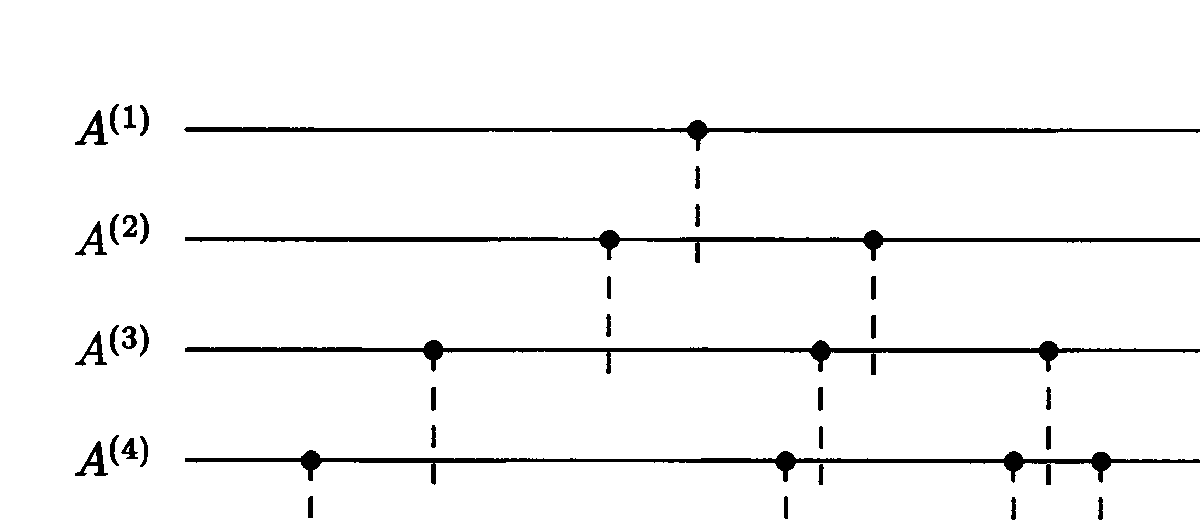
\includegraphics[width=0.86\textwidth]{../assets/figure-30-interlace.png}
\parbox{0.86\textwidth}{\small 图 30.1. 不可约三对角实对称矩阵 $A$ 的主子矩阵 $\{A^{(k)}\}$ 所满足的严格特征值交错性质 (30.6) 示意图。$A^{(k)}$ 的特征值交错于 $A^{(k+1)}$ 的特征值之间；二分法利用了这一性质。}
\end{figure}

正是交错性质使我们能够计算矩阵在指定区间内的特征值个数。例如，考虑三对角
矩阵

$$
A=\begin{bmatrix}
1&1&0&0\\
1&0&1&0\\
0&1&2&1\\
0&0&1&-1
\end{bmatrix}.
$$

由

$$
\det(A^{(1)})=1,\qquad
\det(A^{(2)})=-1,\qquad
\det(A^{(3)})=-3,\qquad
\det(A^{(4)})=4,
$$

可知 $A^{(1)}$ 没有负特征值，$A^{(2)}$ 有一个负特征值，$A^{(3)}$ 有一个
负特征值，而 $A^{(4)}$ 有两个负特征值。

一般地，对任意对称三对角矩阵 $A\in\mathbb{R}^{m\times m}$，负特征值的个数
等于序列

\begin{equation}
1,\ \det(A^{(1)}),\ \det(A^{(2)}),\ \ldots,\ \det(A^{(m)})
\tag{30.7}
\end{equation}

中的符号变化次数；这个序列称为 Sturm 序列。即使中途出现零行列式，这个规则
仍然成立，只要把“符号变化”定义为从正数或 0 变为负数，或从负数或 0 变为正数，
但不把从正数或负数变为 0 计作符号变化。把 $A$ 平移一个单位矩阵的倍数，就
可以确定任意区间 $[a,b)$ 中的特征值个数：它等于 $(-\infty,b)$ 中的个数减去
$(-\infty,a)$ 中的个数。

再观察一点，二分法的描述就完整了：对三对角矩阵，矩阵 $\{A^{(k)}\}$ 的行列式
满足三项递推关系。根据 (30.5)，沿第 $k$ 行对 $\det(A^{(k)})$ 关于
$b_{k-1}$、$a_k$ 的条目作余子式展开，可得

\begin{equation}
\det(A^{(k)})
 =a_k\det(A^{(k-1)})-b_{k-1}^2\det(A^{(k-2)}).
\tag{30.8}
\end{equation}

引入移位 $xI$，并记

$$
p^{(k)}(x)=\det(A^{(k)}-xI),
$$

得到

\begin{equation}
p^{(k)}(x)=(a_k-x)p^{(k-1)}(x)-b_{k-1}^2p^{(k-2)}(x).
\tag{30.9}
\end{equation}

若定义 $p^{(-1)}(x)=0$、$p^{(0)}(x)=1$，那么这个递推对所有
$k=1,2,\ldots,m$ 都成立。

对一系列 $x$ 应用 (30.9)，并沿递推过程统计符号变化，二分法就能把特征值定位到
任意小的区间内。每次计算整个序列需要 $O(m)$ 次浮点运算，因此把一个特征值
求到相对精度 $\varepsilon_{\mathrm{machine}}$ 的总成本为

$$
O\!\left(m\log\frac{1}{\varepsilon_{\mathrm{machine}}}\right)
$$

次浮点运算。如果只需要少量特征值，这相对于 QR 算法的 $O(m^2)$ 运算量是明显
的改进。在多处理器计算机上，还可以让不同处理器独立寻找不同的特征值。

\section*{分治算法}

分治算法通过把对称三对角特征值问题递归地划分为更小维数的问题，代表了自
20 世纪 60 年代以来矩阵特征值算法最重要的进展。这个方法由 Cuppen 于 1981 年
首次提出；如果既需要特征值又需要特征向量，它的速度超过 QR 算法的一倍。

下面只给出核心思想，省略所有细节。不过需要提醒读者：在这个问题中，细节
尤其重要。只有把细节处理正确，算法才是完全稳定的；Cuppen 的原始论文发表后，
这一点甚至十年间都没有被充分理解。

令 $T\in\mathbb{R}^{m\times m}$，$m\ge2$，是实对称、三对角且不可约的矩阵，
即其下对角线只有非零元（否则可以降阶）。对于任意 $1\le n<m$，令 $T_1$ 为
$T$ 左上角的 $n\times n$ 主子矩阵，$T_2$ 为右下角的 $(m-n)\times(m-n)$
主子矩阵，并令

$$
\beta=t_{n+1,n}=t_{n,n+1}\ne0.
$$

记 $e_n$ 为 $\mathbb{R}^n$ 的最后一个标准基向量，记 $e_1$ 为
$\mathbb{R}^{m-n}$ 的第一个标准基向量。将 $T_1$ 的右下角条目替换为
$t_{nn}-\beta$，得到 $\widehat T_1$；将 $T_2$ 的左上角条目替换为
$t_{n+1,n+1}-\beta$，得到 $\widehat T_2$。于是有分裂公式

\begin{equation}
T=
\begin{bmatrix}T_1&\beta e_ne_1^T\\\beta e_1e_n^T&T_2\end{bmatrix}
=
\begin{bmatrix}\widehat T_1&0\\0&\widehat T_2\end{bmatrix}
+\beta
\begin{bmatrix}e_n\\e_1\end{bmatrix}
\begin{bmatrix}e_n\\e_1\end{bmatrix}^{T}.
\tag{30.10}
\end{equation}

也就是说，三对角矩阵可以写成一个带三对角块的 $2\times2$ 分块对角矩阵，加上
一个秩一修正。

分治算法把 $n$ 取为约 $m/2$，按 (30.10) 分裂矩阵 $T$。假设 $\widehat T_1$、
$\widehat T_2$ 的特征值已经知道，由于修正矩阵是秩一的，就可以用一个非线性但
很快的计算，从这两个矩阵的特征值得到 $T$ 的特征值。随后递归应用这一想法，
通过带秩一修正的进一步分裂来求出 $\widehat T_1$、$\widehat T_2$ 的特征值，
如此继续。这样，一个 $m\times m$ 特征值问题就被化为一组 $1\times1$ 特征值
问题和一系列秩一修正。（在实际中，为了获得最大效率，当子矩阵维数足够小时，
通常会切换到 QR 算法，而不会把递归一直进行到底。）

这个过程中有一个关键的数学点：如果 $\widehat T_1$、$\widehat T_2$ 的特征值
已经知道，如何得到 $T$ 的特征值？假设已经计算出对角化

$$
\widehat T_1=Q_1D_1Q_1^T,
\qquad
\widehat T_2=Q_2D_2Q_2^T.
$$

由 (30.10) 可得

\begin{equation}
T=
\begin{bmatrix}Q_1&0\\0&Q_2\end{bmatrix}
\left(
\begin{bmatrix}D_1&0\\0&D_2\end{bmatrix}
+\beta zz^T
\right)
\begin{bmatrix}Q_1^T&0\\0&Q_2^T\end{bmatrix},
\tag{30.11}
\end{equation}

其中 $z^T=(q_1^T,q_2^T)$，$q_1^T$ 是 $Q_1$ 的最后一行，$q_2^T$ 是
$Q_2$ 的第一行。由于这是一个相似变换，问题已经被化为求一个对角矩阵加秩一
修正的特征值。

为说明这一点，简化记号。设要寻找 $D+ww^T$ 的特征值，其中
$D\in\mathbb{R}^{m\times m}$ 是对角矩阵，对角条目 $\{d_j\}$ 互异，
$w\in\mathbb{R}^m$ 是向量。（上面的 $\beta>0$ 时取加号；若 $\beta<0$，
则考虑 $D-ww^T$。）可以假设所有 $w_j\ne0$，否则问题是可约的。那么
$D+ww^T$ 的特征值是有理函数

\begin{equation}
f(\lambda)=1+\sum_{j=1}^{m}\frac{w_j^2}{d_j-\lambda}
\tag{30.12}
\end{equation}

的根，如图 30.2 所示。

\begin{figure}[H]
\centering
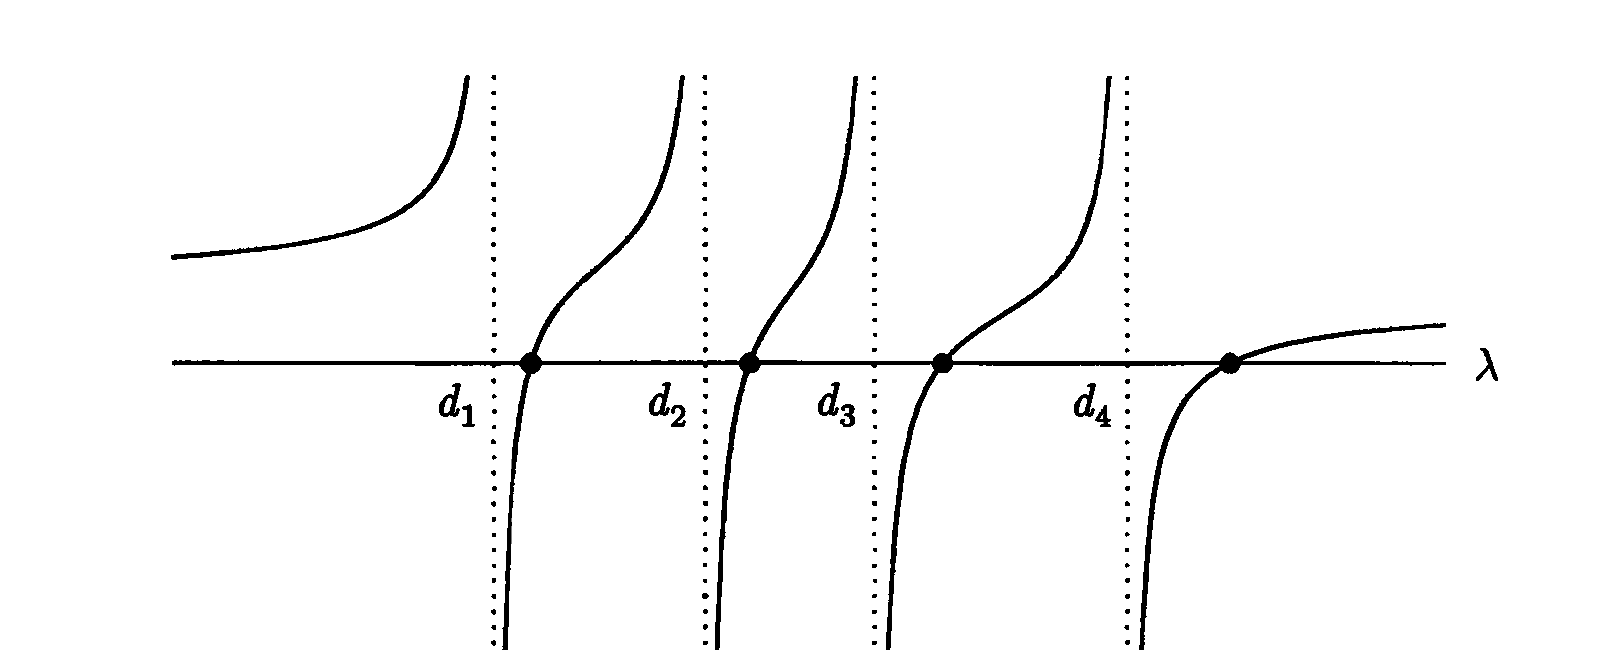
\includegraphics[width=0.94\textwidth]{../assets/figure-30-secular-function.png}
\parbox{0.94\textwidth}{\small 图 30.2. 维数为 4 的问题中式 (30.12) 的函数 $f(\lambda)$。$f(\lambda)$ 的极点是 $D$ 的特征值 $\{d_j\}$，而 $f(\lambda)$ 的根（实心点）是 $D+ww^T$ 的特征值。快速求出这些根，是分治算法每个递归步骤的基础。}
\end{figure}

证明这一点。若对某个 $q\ne0$ 有
$(D+ww^T)q=\lambda q$，则

$$
(D-\lambda I)q+w(w^Tq)=0,
$$

从而

$$
q+(D-\lambda I)^{-1}w(w^Tq)=0.
$$

左乘 $w^T$，得到

$$
w^Tq+w^T(D-\lambda I)^{-1}w(w^Tq)=0,
$$

也就是 $f(\lambda)(w^Tq)=0$。其中 $w^Tq$ 必须非零；否则 $q$ 会成为 $D$ 的
特征向量，即只有一个位置非零，这反过来又会推出 $w^Tq\ne0$。因此，如果
$q$ 是 $D+ww^T$ 的特征值为 $\lambda$ 的特征向量，那么必有 $f(\lambda)=0$。
反过来，由 $f$ 的形式可知它恰有 $m$ 个根，所以结论也成立。方程
$f(\lambda)=0$ 称为 secular 方程。

在分治算法的每个递归步骤中，使用与 Newton 方法有关的快速迭代过程求出
(30.12) 的根。每个根只需要 $O(1)$ 次迭代（如果把
$\varepsilon_{\mathrm{machine}}$ 视为变量，则为
$O(\log|\log\varepsilon_{\mathrm{machine}}|)$ 次），因此对一个
$m\times m$ 矩阵，每个根需要 $O(m)$ 次浮点运算，全部根需要 $O(m^2)$ 次。
若假设递归每一步都把维数准确减半，那么求三对角矩阵特征值的总运算量为

\begin{equation}
O\!\left(m^2+2\left(\frac m2\right)^2
 +4\left(\frac m4\right)^2
 +8\left(\frac m8\right)^2
 +\cdots+m\left(\frac m m\right)^2\right),
\tag{30.13}
\end{equation}

这个级数由于分母中的平方而收敛到 $O(m^2)$，而不是 $O(m^2\log m)$。因此，
表面上看，分治算法与 QR 算法的运算量是同阶的 $O(m^2)$。

到这里，分治算法为什么有优势还不明显。因为把满矩阵约化为三对角形式（第 25 讲
称为“第一阶段”）需要 $4m^3/3$ 次浮点运算（式 (26.2)），看起来即使改进三对角
矩阵对角化（“第二阶段”）的 $O(m^2)$ 运算量，意义也不大。然而，如果同时计算
特征向量，经济性就发生了变化。此时第一阶段需要 $8m^3/3$ 次浮点运算，而第二
阶段也需要 $O(m^3)$ 次：对 QR 算法约为 $6m^3$。分治算法之所以能降低这个数，
根本原因是它的非线性迭代只涉及标量函数 (30.12)，而不涉及正交矩阵 $Q_j$；
QR 算法却必须在每次迭代中处理矩阵 $Q_j$。

运算量分析给出如下结果。分治计算中 $O(m^3)$ 的部分来自 (30.11) 中与 $Q_j$
和 $Q_j^T$ 的乘法。把递归所有层次加起来，总运算量为 $4m^3/3$，相较于
约 $6m^3$ 有很大改进。再加上第一阶段的 $8m^3/3$，总运算量从约 $9m^3$
降到 $4m^3$。

实际上，分治算法通常还能做得更好，原因并不初等。对大多数矩阵 $A$，(30.11)
中出现的许多向量 $z$ 和矩阵 $Q_j$ 都会呈现数值稀疏性，即许多条目的相对大小
小于机器精度。这种稀疏性允许进行数值降阶，把接连出现的三对角特征值问题化为
彼此解耦的更小问题。在典型情况下，这会把第二阶段的运算量降到低于 $m^3$ 的
量级，从而使第一、第二阶段合计为 $8m^3/3$。如果只计算特征值，(30.13) 还是
一个高估，第二阶段的运算量会降到低于 $m^2$ 的量级。这个迷人现象的根源——
本讲不再展开——是大多数三对角矩阵的大多数特征向量都具有“指数局部化”性质
（习题 30.7）；物理学家还把这一事实与玻璃透明的现象联系起来。

我们前面仿佛在谈论一个唯一的分治算法，但实际上存在许多变体。出于稳定性原因，
常常使用更复杂的秩一更新，有时也使用秩二更新；求 $f(\lambda)$ 的根有各种
方法；当 $m$ 很大时，用多极展开来完成与 $Q_j$ 的乘法会比直接算法快。LAPACK
库中提供了高质量的分治算法实现。

\section*{习题}

\paragraph{30.1.}
推导公式 (30.4)，并给出基于该 $\theta$ 选择的变换 (30.1) 的精确几何解释。

\paragraph{30.2.}
Jacobi 算法的一步 (30.1) 需要多少次浮点运算？$m(m-1)/2$ 步，即一轮扫描，
需要多少次浮点运算？这一轮扫描的运算量与先把实对称矩阵三对角化、再用 QR
算法求其特征值的总运算量相比如何？

\paragraph{30.3.}
证明：如果 Jacobi 算法每一步都消去绝对值最大的非对角条目，那么非对角条目
平方和每一步至少缩小为原来的

$$
1-\frac{2}{m^2-m}.
$$

\paragraph{30.4.}
设 $m$ 为偶数，且计算机有 $m/2$ 个处理器。若所用的行/列对为互不相交的

$$
(1,2),(3,4),(5,6),\ldots,(m-1,m),
$$

说明如何并行执行 $m/2$ 个变换 (30.1)。

\paragraph{30.5.}
编写程序，用标准的按行顺序 Jacobi 算法求 $m\times m$ 实对称矩阵的特征值，
并在对数尺度上绘制非对角条目平方和随扫描轮数变化的曲线。对维数为 20、40、
80 的随机矩阵运行程序。

\paragraph{30.6.}
矩阵

$$
A=\begin{bmatrix}
1&1&0&0\\
1&1&1&0\\
0&1&2&1\\
0&0&1&3
\end{bmatrix}
$$

在区间 $[1,2]$ 内有多少个特征值？利用递推式 (30.9)，在纸上通过二分法求出答案。

\paragraph{30.7.}
构造一个维数为 100 的随机实对称三对角矩阵 $T$，并计算其特征值分解
$T=QDQ^T$。在对数尺度上绘制几个特征向量（即 $Q$ 的若干列的绝对值），
观察局部化现象。$Q$ 的 10,000 个条目中，有多大比例的绝对值大于 $10^{-10}$？
如果不用随机矩阵，而使用条目为 $1,-2,1$ 的离散 Laplacian，答案又是什么？

\end{document}
